\documentclass[tikz, margin=3mm]{standalone}
\usetikzlibrary{matrix, fit, chains, arrows.meta, shapes.arrows,
    decorations.pathreplacing,positioning,arrows, positioning} 
% \usepackage[subpreambles=true]{standalone}
% \usepackage[utf8]{inputenc}
% \usepackage[english]{babel}
% \usepackage{import}
\usepackage{array,multirow}
\usepackage{amsmath}
\usepackage{bm}
\usepackage{ifthen}
\usepackage{pgffor}
% \usetikzlibrary{chains, decorations.pathreplacing, positioning}
% \usepackage[dvipsnames]{xcolor}
\definecolor{tab10blue}{RGB}{31, 119, 180}
\definecolor{tab10orange}{RGB}{255, 127, 14}
\definecolor{tab10green}{RGB}{44, 160, 44}
\definecolor{tab10red}{RGB}{214, 39, 40}
\definecolor{tab10purple}{RGB}{148, 103, 189}
\definecolor{tab10brown}{RGB}{140, 86, 75}
\definecolor{tab10pink}{RGB}{227, 119, 194}
\definecolor{tab10gray}{RGB}{127, 127, 127}
\definecolor{tab10olive}{RGB}{188, 189, 34}
\definecolor{tab10cyan}{RGB}{23, 190, 207}
\definecolor{myBlue}{RGB}{0, 157, 248}
\definecolor{myRed}{RGB}{255, 96, 96}
\definecolor{myGreen}{RGB}{21, 173, 87}
\definecolor{darkB}{RGB}{26, 78, 102}
\definecolor{lightB}{RGB}{166, 212, 241}
\definecolor{darkG}{RGB}{38, 133, 120}
\tikzset{%
square matrix/.style={
    matrix of nodes,
    column sep=-\pgflinewidth, 
    row sep=-\pgflinewidth,
    nodes in empty cells,
    nodes={rectangle, draw,    
      minimum height=2em, minimum width=2em,
      fill=white,
      anchor=center,
      align=center,
      inner sep=0pt, outer sep=0pt
    }
},
square matrix/.default=0.5cm,
}
\begin{document}
\pagestyle{empty}
\sffamily
\def\layersep{2.5cm}
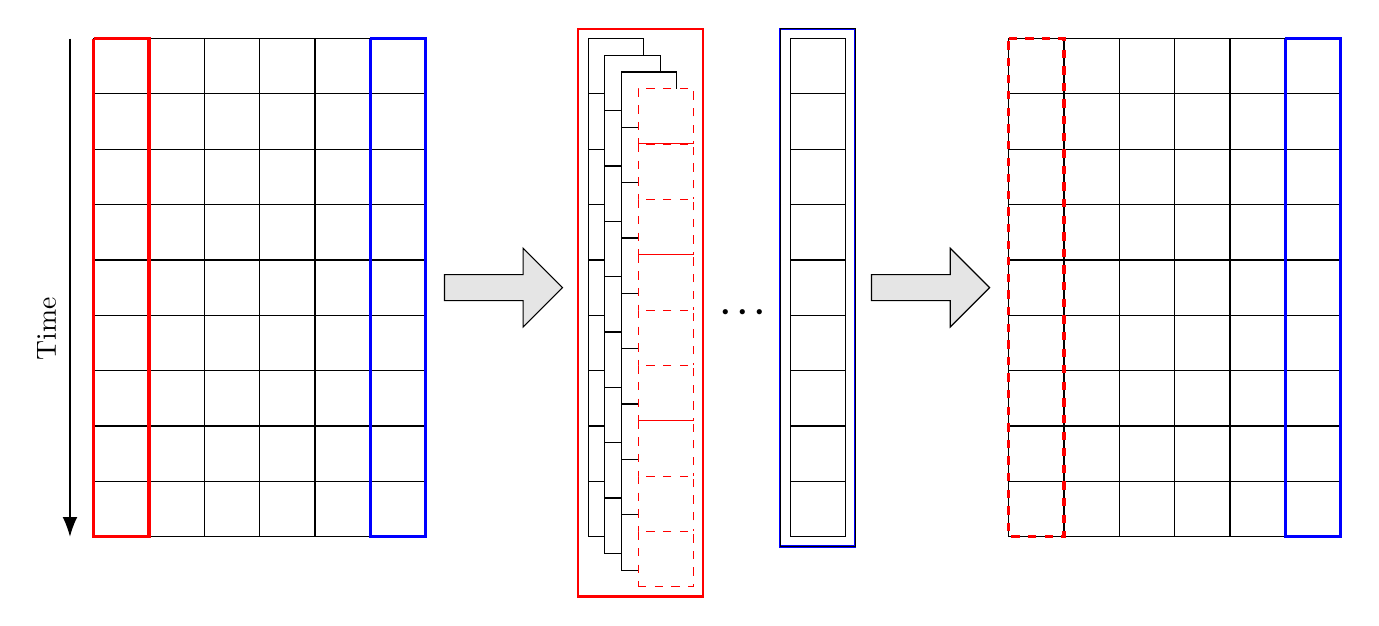
\begin{tikzpicture}[]

\matrix[square matrix] (ts)
{
  & & & & & \\ 
  & & & & & \\ 
  & & & & & \\ 
  & & & & & \\ 
  & & & & & \\ 
  & & & & & \\ 
  & & & & & \\ 
  & & & & & \\ 
  & & & & & \\ 
};]
\draw [-{Latex[length=2.5mm]}] (ts-1-1.north west)++(-0.3,0) coordinate (temp) 
            -- (temp |- ts-9-1.south) node[midway,anchor=east,xshift=-0.3cm,rotate=90]{Time};
\draw [very thick, red] (ts-1-1.north west) -- (ts-1-1.north east) -- (ts-9-1.south east) -- (ts-9-1.south west) -- (ts-1-1.north west) ;
\draw [very thick, blue] (ts-1-6.north west) -- (ts-1-6.north east) -- (ts-9-6.south east) -- (ts-9-6.south west) -- (ts-1-6.north west) ;

\node (sea-arrow) [single arrow,draw=black,fill=black!10,right=0.1cm of ts,minimum height=1.5cm,minimum width=1cm] {};
% first column
\begin{scope}[local bounding box=ts-col1]
\matrix[square matrix, right=1.8cm of ts] (ts-col1-y) { \\ \\  \\  \\  \\  \\  \\  \\  \\ };]
\matrix[square matrix, below right=0.3cm of ts-col1-y.north west] (ts-col1-w){ \\ \\  \\  \\  \\  \\  \\  \\  \\ };]
\matrix[square matrix, below right=0.3cm of ts-col1-w.north west] (ts-col1-h){ \\ \\  \\  \\  \\  \\  \\  \\  \\ };]
\matrix[square matrix, red,dashed,below right=0.3cm of ts-col1-h.north west] (ts-col1-r){ \\ \\  \\  \\  \\  \\  \\  \\  \\ };]
\end{scope}
\draw [thick, red] (ts-col1.south west) rectangle (ts-col1.north east);
% \draw[pattern=north west lines, pattern color=blue] (0,0) rectangle (2,4);
\node (col_dots) [right=0.1cm of ts-col1,text width=1cm,font=\bfseries] {\large $\bm{\cdots}$}; 
% last column
\begin{scope}[local bounding box=ts-coln]
\matrix[square matrix, right=1.6cm of ts-col1-y.east] (ts-coln-y) { \\ \\  \\  \\  \\  \\  \\  \\  \\ };]
\end{scope}
\draw [thick, blue] (ts-coln.south west) rectangle (ts-coln.north east);
\node [fit=(ts-coln),inner sep=0pt,draw] {};

\node (sea-arrow2) [single arrow,draw=black,fill=black!10,right=0.2cm of ts-coln,minimum height=1.5cm,minimum width=1cm] {};
\matrix[square matrix, right=0.1cm of sea-arrow2] (ts2)
{
  & & & & & \\ 
  & & & & & \\ 
  & & & & & \\ 
  & & & & & \\ 
  & & & & & \\ 
  & & & & & \\ 
  & & & & & \\ 
  & & & & & \\ 
  & & & & & \\ 
};]
\draw [very thick, dashed, red] (ts2-1-1.north west) -- (ts2-1-1.north east) -- (ts2-9-1.south east) -- (ts2-9-1.south west) -- (ts2-1-1.north west) ;
\draw [very thick, blue] (ts2-1-6.north west) -- (ts2-1-6.north east) -- (ts2-9-6.south east) -- (ts2-9-6.south west) -- (ts2-1-6.north west) ;
\end{tikzpicture}
% End of code
\end{document}